% This is samplepaper.tex, a sample chapter demonstrating the
% LLNCS macro package for Springer Computer Science proceedings;
% Version 2.20 of 2017/10/04
%
\documentclass[runningheads]{llncs}
%
\usepackage{graphicx}
\usepackage[portuges]{babel}
\usepackage[T1]{fontenc}
\usepackage{verbatim}
\usepackage{float}
\usepackage{caption}
%Path relative to the .tex file containing the \includegraphics command
\graphicspath{ {./images/} }
% Used for displaying a sample figure. If possible, figure files should
% be included in EPS format.
%
% If you use the hyperref package, please uncomment the following line
% to display URLs in blue roman font according to Springer's eBook style:
% \renewcommand\UrlFont{\color{blue}\rmfamily}
\setcounter{secnumdepth}{6}
\renewcommand\theparagraph{\Alph{paragraph}}
 
\makeatletter
\renewcommand\paragraph{\@startsection{paragraph}{4}{\z@}%
                                      {-3.25ex\@plus -1ex \@minus -.2ex}%
                                      {0.0001pt \@plus .2ex}%
                                      {\normalfont\normalsize\bfseries}}
\renewcommand\subparagraph{\@startsection{subparagraph}{5}{\z@}%
                                      {-3.25ex\@plus -1ex \@minus -.2ex}%
                                      {0.0001pt \@plus .2ex}%
                                      {\normalfont\normalsize\bfseries}}
 
\counterwithin{paragraph}{subsubsection}
\counterwithin{subparagraph}{paragraph}
\makeatother

\begin{document}
%
\title{CMD-SOAP - Teste das operações do serviço SCMD}
%
\titlerunning{Teste das operações do serviço SCMD}
% If the paper title is too long for the running head, you can set
% an abbreviated paper title here
%
\author{ Henrique José Carvalho Faria nº82200 }
%
% First names are abbreviated in the running head.
% If there are more than two authors, 'et al.' is used.
%
\institute{Departamento de Informática, Universidade do Minho}
%
\maketitle              % typeset the header of the contribution
%
% Abstract
\begin{abstract}


Neste trabalho foi-nos pedido que emulássemos o programa \textit{CMD-SOAP} desenvolvido pelo professor em \textit{Perl}. Adicionalmente este programa deve aplicar medidas de segurança que previnam diversos ataques que podem ser realizados por idividuos mal intencionados. Assim, começamos por emular o programa, seguindo-se um estudo das vulnerabilidades mais prováveis de ocorrerem em programas bem como das vulnerabilidades mais conhecidas de programas \textit{Perl}.
Assim este relatório começa por descrever o processo de emulação da aplicação e posteriormente realiza uma sumula das vulnerabilidades possíveis e de que forma foram tratadas.


\keywords{Perl \and Buffer-Overflow \and String Vulnerabilitys \and Integer Vulnarabilitys \and Input Validation \and white List}
\end{abstract}
%
%








\newpage
\newpage
\hfill
% Aqui começam os capitulos abordados pelo trabalho
\section{Criação da aplicação CMD-SOAP em Perl}

Para este trabalho seguiu-se a estrutura do programa original separando o corpo da aplicação, que ficou no ficheiro test\_cmd\_wsdl.pl, das operações sobre ficheiros, chave móvel e ligação ao servidor, que ficaram no modulo cmd\_soap\_msg.pm, e da variável APPLICATION\_ID que ficou no modulo cmd\_config.pm. Adicionalmente foi criado um módulo para tratamento de segurança da aplicação chamado \textit{verifiers.pm}.\newline


Para o corpo do programa o Perl começa por importar a variável \textit{\$APPLICATION\_ID} do modulo \textit{cmd\_config} através da subrotina \textit{get\_appid()}. Caso esta variável não esteja definida o programa termina. \newline
Em seguida é verificado se o programa foi invocado com argumentos, caso contrário o programa também termina. Caso tenha sido invocado com argumentos é realizado um parser dos dados recorrendo ao módulo \textit{Getopt::Long} que faz uso de flags para identificar inequivocamente cada variável recebida como parâmetro. Em seguida estes argumentos são colecionados num array cujas variáveis definidas serão verificadas fazendo uso das subrotinas pertencentes ao módulo \textit{verifiers.pm}.\newline
Caso o input passe nas verificações de segurança, o pedido do cliente é passado ao módulo \textit{cmd\_soap\_msg.pm} e dependendo do tipo de operação pedida pelo utilizador é chamada a respetiva subrotina. Caso o utilizador pretenda testar todo o programa pode usar a operação \textit{test} que corre todas as subrotinas por ordem de forma a realizar a assinatura com a chave móvel digital sobre o ficheiro fornecido.\newline
Convêm referir que, ao contrário do que foi realizado no ficheiro original \textit{test\_cmd\_wsdl.py} as verificações de segurança referentes ao código das mensagens recebidas do servidor foram realizados no módulo \textit{cmd\_soap\_msg.pm}.

\subsection{Módulos}

Para instalar os módulos necessários pode-se utilizar uma ferra menta chamada \textit{cpanm}. Pode-se descarregar esta ferramenta para linux com o comando de terminal \textit{sudo apt install cpanminus}.\newline
Após instalar a ferramenta deve-se garantir que se tem os seguintes módulos instalados\footnote{Nota: Para descarregar os módulos use no terminal o comando cpanm install 'nome do módulo'}:

\begin{enumerate}
	\item XML::Compile::WSDL11
	\item XML::Compile::SOAP11
	\item XML::Compile::Transport::SOAPHTTP
	\item Encode
	\item Bit::Vector
	\item Digest::SHA
	\item HTTP::Request
	\item HTTP::Parser
	\item MIME::Base64
	\item File::Basename
	\item File::Slurp
	\item Try::Tiny
	\item Getopt::Long
	\item Switch
	\item File::Basename
	\item Crypt::OpenSSL::X509
	\item Crypt::PK::RSA
	\item Crypt::Misc
	\item Carp::Assert
\end{enumerate}

\newpage
\section{Vulnerabilidades Gerais}

No desenvolvimento de um software devemos sempre garantir que não divulgamos informação sobre como a nossa aplicação está construida. Durante o deenvolvimento do código deparamo-nos com dois possíveis problemas a tratar.\newline
\par O primeiro problema enuncia-se em seguida, "Como encerrar a aplicação com uma exceção passando uma mensagem de erro ao utilizador sem lhe revelar informação sobre o código da aplicação?". Para resolver este problema usamos a função \textit{die}, o problema é que esta para além da mensagem fornece informação sobre a linha onde ocorreu a exceção. Felizmente caso se adicione \textit{\\n} ao final da mensagem de erro emitida pelo die este omite a informação referente á linha. 
\par O segundo problema encontrado é referente á função \textit{open}, até ao ano 2000, a função open usava 2 parâmetros, um para a variável para a qual se lê e uma para o ficheiro a ler. O problema  acontece caso o utilizador use um ficheiro cujo nome comece, por exemplo, com o sinal \textit{>}, isto levará a que por exemplo caso seja dado como input o ficheiro \textit{>/etc/passwd} nós acabamos de apagar o ficheiro de passwords do Linux. Para resolver este problema usamos a versão do open com 3 variáveis, uma para guardar a informação a ler do ficheiro, uma para o tipo de leitura a realizar no ficheiro e uma para o nome do ficheiro. Acresce a este problema o facto de que caso o open use um pipe em vez de um ficheiro, ao falhar este devolve o pid do subprocesso na mensagem de erro, como queremos evitar divulgar qualquer informação sobre a aplicação usamos então a função \textit{die} para emitir o erro sem comprometer a nossa implementação tomando o código a seguinte forma: \textit{open(variável para leitura, modo de leitura, ficheiro a ler) or die ... }.\newline

\textit{Nota: As restantes questões de segurança foram abordadas e tratadas num modulo perl a parte chamado \textbf{verifiers.pm} criado para separar de forma legivel as subrotinas usadas para segurança das subrotinas do programa principal.}\newline 

Existem enúmeras vulnerabilidades a tratar para além das duas supramencionadas, nomeadamente:
\begin{enumerate}
\item Restrições sobre a memória
\item Neutralização do input durante a geração da página web
\item Improper Input Validation
\item Information Exposure
\item Out-of-Bounds Read
\item Neutralização de elementos especiais para comandos SQL (SQL Injection)
\item use after free
\item Integer Overflow or Wrapparound
\item XML Injection
\item OS Commands Injection
\item SQL Injection
\end{enumerate}

Destas vulnerabilidades a 1ª 4ª, 5ª, 6ª, 7ª e 8ª podem ser ignoradas visto que o \textit{Perl} trata da alocar as variáveis na memória libertando o programador da manutenção da mesma, para além. Assim vamos debruçar-nos sobre a vulnerabilidade 3, 9,10 e 11.


\subsection{Improper Input Validation}

Nesta secção falaremos um pouco dos inputs e da validação realizada sobre os mesmos. A validação de inputs de uma aplicação é fulcral para o bom funcionamento da mesma, nunca devemos acreditar que o utilizador usará a aplicação da melhor forma ou para fins nefastos.\newline
Assim os inputs a verificar são: o nome do ficheiro, o número de telefone, o pin, o OTP e o process Id.\newline

\begin{itemize}
\item Nome do ficheiro\newline
 Para realizar a verificação do nome do ficheiro foram criadas 2 listas, uma white list com os caracters aceitaveis para constituirem o nome de um ficheiro (As White Lists são especialmente proveitosas visto que é mais facil indicar o que é aceitavel do que o que não é, em contrapartida limitamos um pouco os nomes possíveis para os ficheiros fornecidos) e uma black list onde removemos algumas hipóteses aceitáveis na white list mas que não podem ser dados como input do nome do ficheiro que são as flags usadas nos inputs do programa.\newline
 Convem notar que tentativas de inserção de vários comandos através da adição de \textit{;} ou de pipes com o caracter \textit{|} não funcionam pois não pertencem á lista de caracters permitidos pela white list.

\hfill\newline
\item Número de telefone\newline
 No caso do número de telefone desenvolvemos 2 regex sendo que um funciona para números internacionais e nacionais e um que funciona apenas para números nacionais, os respetivos regex apresentam-se em seguida:\newline
\begin{itemize}
	\item \textit{/\^{}\textbackslash+[0-9]\{1,3\} [0-9]\{4,14\}\$/}
	\item \textit{/\^{}\textbackslash+351 [0-9]\{9\}\$/}
\end{itemize}

\hfill\newline
\par Como a chave móvel digital para a qual a aplicação se destina normalmente está associada a números de telemovel portugueses mantivemos o segundo regex embora tenhamos deixado em comentário o segundo regex caso pretendamos estender a aplicação a números estrangeiros. A razão de escolhermos apenas números nacionais prende-se com a esolha de implementar uma segurança com granularidade mais fina visto que o número de dígitos de telemovel varia de país para país e o indicativo também.\newline
\textit{Nota: Convem notar que, nas expressões regex, são usados por vezes 2 simbolos, o \^{} no inicio do regex e o \$ no fim. Estes simbolos indicam ao perl que o regex tem de corresponder ao inicio do input e ao final deste respetivamente, isto é, caso ambos os simbolos sejam usados o perl entende que o input a testar tem de ser totalmente formado pelo regex e, caso não seja, falha a verificação.}\newline
\hfill\newline
\item PIN\newline

\par O PIN é um conjunto de 4 digitos, assim, para o testar bastou um regex simples que garantisse isso: \textit{/\^{}[0-9]\{4\}\$/}.

\hfill\newline
\item OTP\newline
\par O OTP é verificado como endo um conjunto de 6 digitos. Mais uma vez o regex usado é bastante simples: \textit{/\^{}[0-9]\{6\}\$/}.

\end{itemize}


O principal foco da segurança na nossa aplicação foi aplicado ás strings. Os critérios usados na \textit{white List} e na \textit{Black List} não são muito restritivos, principalmente porque as strings são maleáveis e o utilizador pode dar o nome que quiser ao documento que pretende utilizar com a aplicação. Desta forma é necessário ter atenção a utilizadores mal intencionados que pretendam usar os critérios laços de filtragem de input para fins diferentes daquele para o qual a aplicação foi feita.\newline


\subsection{OS Injection}

O Perl é relativamente suscetivel a injeção de comandos do sistema operativo, isto pois permite utilizar pipelines com o caracter \textit{|} como input ou comandos seguidos separados pelo caracter \textit{;}. Para ambos os casos existe uma solução que apesar de restringir a liberdade do cliente de nomear os seus ficheiros recorrendo aos caracters \textit{|} e \textit{|} garante que estes ataques não ocorrem, o que do ponto de vista de uma maior qualidade na segurança da aplicação é o ideal.


\subsection{XML Injection}

Nesta subsecção vamos tratar de qualquer tentativa de injeção de código \textit{XML} na nossa aplicação. Para lidar com tentativas de injeção de código \textit{XML} através de um input foi criada uma subrotina chamada {xmlInjection} no modulo \textit{verifiers.pm}.\newline
Nesta subrotina para evitar eventuais tentativas de injeção de código \textit{XML} foi realizado um regex com a forma: \textit{/$<$[a-zA-Z]*($>$[\^{} ($<$\textbackslash/)]*$<$/[a-zA-Z]*|\textbackslash/)?$>$/} . Este regex permite realizar match entre elementos desta linguagem através de sintaxe conhecida detetando padrões como \textit{<qualquer coisa> ... </qualquer coisa>} ou \textit{<qualquer coisa/>}.

\subsection{SQL Injection}

Para tratar eventuais tentativas de injeção de código \textit{SQL} através das variáveis, foi definida uma subrotina chamada \textit{sqlInjection} que possui um array de palavras chave usadas na syntax \textit{SQL} que são comparadas através de um regex com os argumentos. Caso seja detetado num argumento uma palavra pertencente á syntax \textit{SQL} o programa emite uma mensagem de erro a avisar que detetou uma tentativa de SQL injection.

\section{Certificados Falsos}

Um problema quando se lida com certificados prende-se com a validação dos mesmos. De forma a contornar este problema recorreu-se ao módulo \textit{LWP::UserAgent}, este fornece uma opção por defeito de verificação automática do servidor e da sua legitimidade chamada \textit{verify\_hostname}. Assim são escolhidos protocolos seguros e é assegurado que nos ligamos a um servidor que possui um certificado válido.

\newpage
\section{Como correr o programa}

Para correr o programa desenvolvido temos várias opções. Para saber qual a sintaxe pela qual o programa se rege deve-se chamar o programa com um argumento ou sem argumentos escrevendo no terminal uma das seguintes opções:
\begin{itemize}
	\item perl test\_cmd\_wsdl.pl
	\item perl test\_cmd\_wsdl.pl -h
\end{itemize} 
\hfill\newline
\par Caso se pretenda saber quais as opções de input disponíveis para cada operação devemos inserir uma das seguintes opções:
\begin{itemize}
	\item perl test\_cmd\_wsdl.pl -o test -h
	\item perl test\_cmd\_wsdl.pl -o gc -h
	\item perl test\_cmd\_wsdl.pl -o ms -h
	\item perl test\_cmd\_wsdl.pl -o mms -h
	\item perl test\_cmd\_wsdl.pl -o otp -h
\end{itemize}
\hfill\newline
Para testar as várias operações basta inserir um dos seguintes comandos no terminal, adicionalmente pode-se escolher se se usa a opção -prod ou não com cada comando:
\begin{itemize}
	\item perl test\_cmd\_wsdl.pl -o test -f  ../LICENCE -u ''user phone number' -p 'your pin'
	\hfill\newline
	\item perl test\_cmd\_wsdl.pl -o gc -otp 'OTP received in your device' -procId 'ProcessID received in the answer of the   CCMovelSign/CCMovelMultipleSign command'
	\hfill\newline
	\item perl test\_cmd\_wsdl.pl -o ms -u 'user phone number' -p 'your pin'
	\hfill\newline
	\item perl test\_cmd\_wsdl.pl -o mms -u 'user phone number' -p 'your pin'
	\hfill\newline
	\item perl test\_cmd\_wsdl.pl -o otp -otp 'OTP received in your device' -procId 'ProcessID received in the answer of the   CCMovelSign/CCMovelMultipleSign command'
\end{itemize}
\newpage
Caso corra a aplicação com o comando \textit{test} o resultado esperado deve ser o seguinte:
\begin{figure}[H]

  \centering
  \captionsetup{justification=centering}

  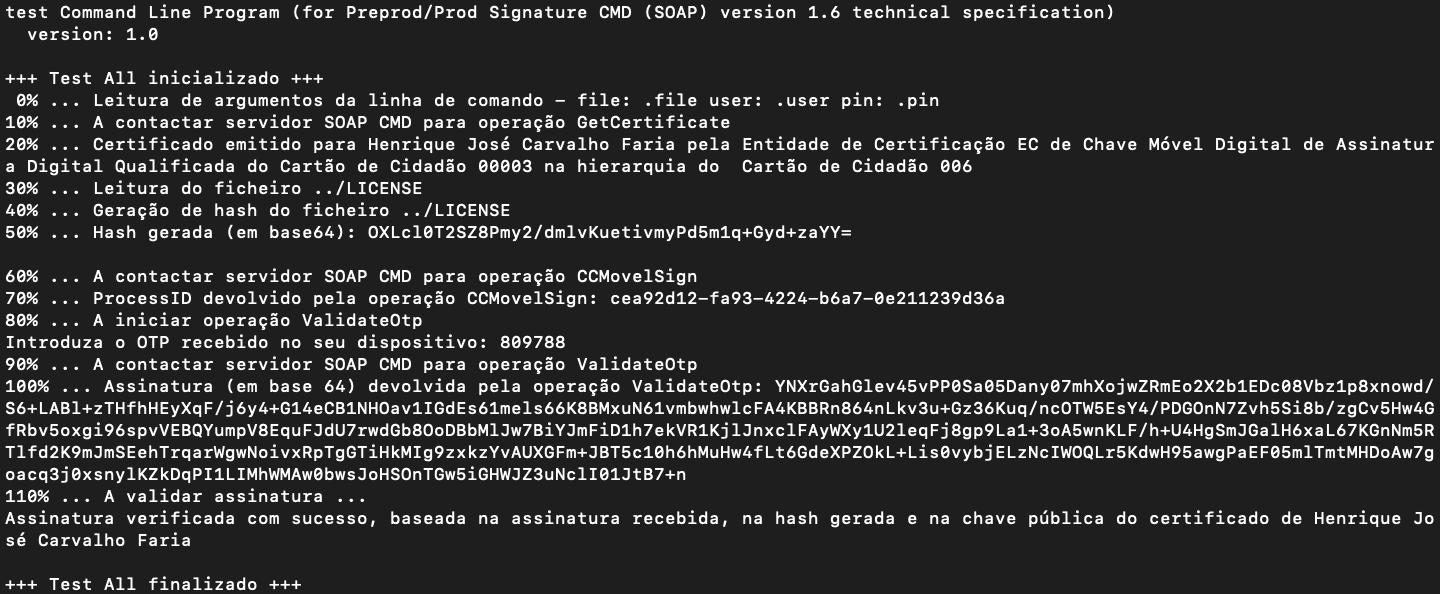
\includegraphics[scale = 0.25]{resultado.png}
  
  \caption {Resultado de correr o comando perl test\_cmd\_wsdl.pl -o test -f  'file name' -u 'user phone number' -p 'your pin' com ou sem a opção prod}

  \label {fig01}

\end{figure}
\newpage
%
% ---- Bibliography ----
%
% BibTeX users should specify bibliography style 'splncs04'.
% References will then be sorted and formatted in the correct style.
%
% \bibliographystyle{splncs04}
% \bibliography{mybibliography}
%
%\begin{thebibliography}{8}

%\bibitem{ref_intro1}
%https://www.itu.int/en/ITU-D/Statistics/Pages/stat/default.aspx


%\end{thebibliography}
\end{document}
